\subsection{Équation différentielle}

\begin{definition}
Un oscillateur harmonique à un degré de liberté est un système dont l'évolution est régie par une grandeur $x(t)$ solution de :
\[\frac{\dif^2 x}{\dif t^2} + {\omega_0}^2 x = 0\]
pour une certain constante $\omega_0$, appelée \tdef{pulsation propre} de l'oscillateur.
\end{definition}

\begin{exemple}
Un object mobile $\systeme{M}$ de masse $m$ fixé en son centre à un ressort horizontal linéaire de raideur $k$, de longueur à vide $l_0$ et de masse négligeable est un oscillateur harmonique lorsque les frottements sont négligés.

\begin{figure}[H]
\begin{center}
\begin{tikzpicture}[thick]
\node (A) at (0,0)   [inner sep=0pt, minimum size=0.3cm]   {};
\node (M) at (4.5,0) [rectangle, schema, minimum size=1cm] {$\systeme{M}$};

\fill [bati] (0,0.5) -- (0,-0.5) -- (6,-0.5) -- (6,-0.7) -- (-0.2,-0.7) -- (-0.2,0.5) -- cycle;
\draw (0,0.5) -- (0,-0.5) -- (6,-0.5);

\draw (A.center) -- (A.east);
\draw [ressort={0.5}{4.5mm}] (A) -- (M);

\draw [<->] (0,0.7) -- node [above] {$\ell_0$} (2.5,0.7);

\draw [->] (0,-1) -- (7,-1);
\foreach \x/\xtext in {2.5/$0$, 4.5/$x$}
\draw [xshift=\x cm, yshift=-1cm] (0,-0.1) -- node [below=0.1] {\xtext} (0,0.1);

\draw [<->] (-2,0) node [above] {$\vecteur{u_y}$} -- (-2,-1) -- (-1,-1) node [right] {$\vecteur{u_x}$};

\draw [->] (6,1) -- node [right] {$\vecteur{g}$} (6,0);
\end{tikzpicture}
\end{center}
\end{figure}

\noindent En effet, l'écart $x$ à la position d'équilibre est alors solution de l'équation de l'oscillateur harmonique de pulsation propre $\omega_0 = \sqrt{\frac{k}{m}}$
\end{exemple}



\subsection{Étude des solutions}

\begin{propriete}
Les solutions de l'équation de l'oscillateur harmonique de pulsation propre $\omega_0$ et d'inconnue $x$ s'écrivent :
\[x(t) = X_m \cos(\omega_0 t + \varphi) \quad \text{ou} \quad x(t) = A \cos(\omega_0 t) + B \sin(\omega_0 t)\]
où les couples $X_m$ et $\varphi$ d'une part, et $A$ et $B$ de l'autre, sont des couples de \tdef{constantes d'intégration} que l'on obtient à l'aide des \imp{conditions initiales}. On passe d'une écriture à l'autre à l'aide des relations :
\[X_m = \sqrt{A^2 + B^2} \quad \text{et} \quad \tan \varphi = - \frac{B}{A}\]
\end{propriete}

\begin{remarque}
La première écriture montre que les solutions sont \imp{sinusoïdales}.
\end{remarque}

\begin{definition}
La \tdef{période propre} $T_0$ d'un oscillateur est définie comme étant la période de ses oscillations :

\begin{figure}[H]
\begin{center}
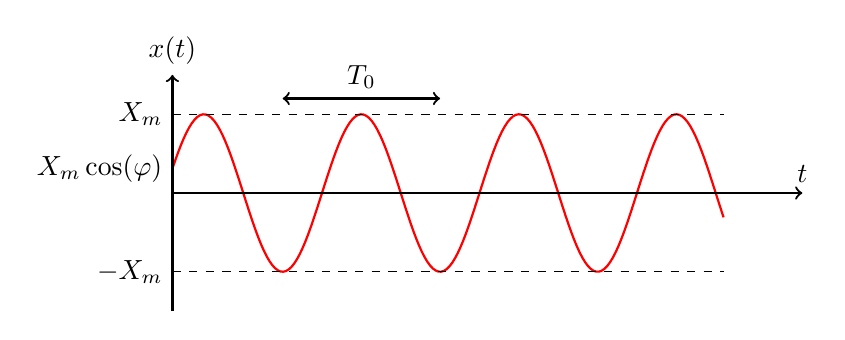
\begin{tikzpicture}[thick, domain=0:7]

\draw [red, variable=\t, samples=200] plot (7-\t,{cos((\t-0.6) * pi r)}) node [left, black] {$X_m \cos(\varphi)$};

\draw [->] (0,-1.5) -- (0,1.5) node [above] {$x(t)$};
\draw [->] (0,0) -- (8,0) node [above] {$t$};

\foreach \x/\xtext in {1/$X_m$, -1/$-X_m$}
\draw [thin,dashed] (0,\x) node [left] {\xtext} -- (7,\x);

\draw [<->] (1.4,1.2) -- node [above] {$T_0$} (3.4,1.2);
\end{tikzpicture}
\end{center}
\end{figure}

\noindent On définit de plus la \tdef{fréquence propre} $f_0 = \frac{1}{T_0}$.
\end{definition}

\begin{propriete}
La période propre $T_0$ s'exprime :
\[T_0 = \frac{2\pi}{\omega_0}\]
On remarque que $T_0$ est indépendante des conditions initiales : on parle d'\tdef{isochronisme des oscillations}.
\end{propriete}



\subsection{Portrait de phase}

\begin{propriete}
Les trajectoires de phase d'un oscillateur harmonique sont des ellipses de demi-axes $X_m$ et $\omega_0 X_m$ :

\begin{figure}[H]
\begin{center}
\begin{tikzpicture}[thick]

\draw [red, decoration={markings, mark=at position 0.125 with {\arrow{<}}, mark=at position 0.625 with {\arrow{<}}}, postaction={decorate}] (0,0) ellipse [x radius=2cm, y radius=4cm/3];

\draw [->] (0,-2) -- (0,2) node [above] {$\dot{x}$};
\draw [->] (-3,0) -- (3,0) node [right] {$x$};

\draw [xshift=2cm] (0,-0.1) -- node [below right=0.1] {$X_m$} (0,0.1);
\draw [yshift=4cm/3] (-0.1,0) -- node [above right=0.1] {$\omega_0 X_m$} (0.1,0);
\end{tikzpicture}
\end{center}
\end{figure}

\end{propriete}